\documentclass[10.5pt,landscape]{article}
\usepackage{ctex}
\usepackage{multicol}
\usepackage{calc}
\usepackage{ifthen}
\usepackage[landscape]{geometry}
\usepackage{amsmath,amsthm,amsfonts,amssymb}
\usepackage{color,graphicx,overpic}
\usepackage{hyperref}
\usepackage{graphicx}
\usepackage{amsmath}
\graphicspath{ {sheet_images/} }

%Originally Modified by Daniel Kenner for Calc 3 Cheat Sheet
%Template Originally found @ http://tex.stackexchange.com/questions/8827/preparing-cheat-sheets
%Conic images originally found on google images when looking for named shapes

% This sets page margins to .5 inch if using letter paper, and to 1cm
% if using A4 paper. (This probably isn't strictly necessary.)
% If using another size paper, use default 1cm margins.
\ifthenelse{\lengthtest { \paperwidth = 11in}}
    { \geometry{top=.25in,left=.25in,right=.25in,bottom=.25in} }
    {\ifthenelse{ \lengthtest{ \paperwidth = 297mm}}
        {\geometry{top=1cm,left=1cm,right=1cm,bottom=1cm} }
        {\geometry{top=1cm,left=1cm,right=1cm,bottom=1cm} }
    }

% Turn off header and footer
\pagestyle{empty}

% Redefine section commands to use less space
\makeatletter
\renewcommand{\section}{\@startsection{section}{1}{0mm}%
                                {-1ex plus -.5ex minus -.2ex}%
                                {0.5ex plus .2ex}%x
                                {\normalfont\large\bfseries}}
\renewcommand{\subsection}{\@startsection{subsection}{2}{0mm}%
                                {-1explus -.5ex minus -.2ex}%
                                {0.5ex plus .2ex}%
                                {\normalfont\normalsize\bfseries}}
\renewcommand{\subsubsection}{\@startsection{subsubsection}{3}{0mm}%
                                {-1ex plus -.5ex minus -.2ex}%
                                {1ex plus .2ex}%
                                {\normalfont\small\bfseries}}
\makeatother

% Define BibTeX command
\def\BibTeX{{\rm B\kern-.05em{\sc i\kern-.025em b}\kern-.08em
    T\kern-.1667em\lower.7ex\hbox{E}\kern-.125emX}}

% Don't print section numbers
\setcounter{secnumdepth}{0}


\setlength{\parindent}{0pt}
\setlength{\parskip}{0pt plus 0.5ex}

%My Environments
\newtheorem{example}[section]{Example}
% -----------------------------------------------------------------------

\begin{document}
\raggedright
\footnotesize
\begin{multicols*}{4}


% multicol parameters
% These lengths are set only within the two main columns
%\setlength{\columnseprule}{0.25pt}
\setlength{\premulticols}{1pt}
\setlength{\postmulticols}{1pt}
\setlength{\multicolsep}{1pt}
\setlength{\columnsep}{2pt}

\textbf{ 噪声} \newline
\scriptsize
$F_n = \frac{SNR_i}{SNR_o}=\frac{P_{no}}{G_p P_{ni}}$\newline
$P_{nim}=kT\Delta f, P_{sim}=\frac{v_s^2}{4R_s}$\newline
无源:$F_n = \frac{1}{G_p}$\newline
级联:$F_n  = F_{n1} + \frac{F_{n2} - 1}{G_{pm1}} + \frac{F_{n3} - 1}{G_{pm1}G_{pm2}} ... $\newline
灵敏度:$P_{si(min)} = SNR_{o min}F_n k_B T \Delta f$ \newline
\textbf{谐振、匹配、部分接入}\newline
$H(s) = A_0[ \frac{1}{Q}\frac{s}{\omega_0}] / [(\frac{s}{\omega_0})^2 + \frac{1}{Q}\frac{s}{\omega_0} + 1]$\newline
$BW = \frac{\omega_0}{2\pi Q} $\newline
$ \phi(\omega) = -arctan Q(\frac{\omega}{\omega_0} - \frac{\omega_0}{\omega}) $\newline
$ \omega_0 = \frac{1}{\sqrt{LC}} $\newline
$ Q = \frac{\omega_0 C}{G} = \frac{1}{\omega_0LG}  = \frac{Y_0}{G} $\newline
$ Z = \omega_0 L = \frac{1}{\omega_0 C} $\newline
有损电感:$ Q = \frac{Z_0}{r_s}, R_p = Q Z_0 = Q \frac{L}{C}$\newline
部分接入:$ R_L' = \frac{R_L}{p^2}, C_L' = p^2 C_L $\newline
$ p = \frac{C_1}{C_1 + C_2}  p = \frac{L2}{L1 + L2} $\newline
变压器:$n = N_1:N_2$则$R_L' = n^2R_L$ \newline
\textbf{L型匹配}\newline
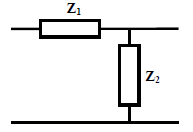
\includegraphics[scale=0.5]{L}\newline
$ R_s = \sqrt{(Z_1 + Z_2)Z_1}, R_L = \sqrt{Z_2 \frac{Z_1 Z_2}{Z_1 + Z_2}}$ \newline
$ Z_1 = \pm jR_S \sqrt{\frac{R_L}{R_S} - 1}$\newline
$ Z_2 = \mp jR_L / \sqrt{\frac{R_L}{R_S} - 1}$ \newline
$ Q = \sqrt{\frac{R_p}{R_s} - 1}$ \newline
$ Q = \frac{1}{\omega R_s C_s} = \omega R_pC_p$ \newline
$ Q = \frac{\omega L_s}{R_s} = \frac{R_p}{\omega L_p}$ \newline
\textbf{双共轭匹配} \newline
双端同时共轭匹配则实现最大功率传输,达到MAG \newline
$\Delta = Re^2(A^*D + B^*C)- | AD - BC |^2$ \newline
$a_1 = Re{C^*D}, a_2 = Re{C^*A}$ \newline
$k = \frac{Re(A^*D + B^*C)}{| AD - BC |} > 1$ \newline
$MAG = \frac{k - \sqrt{k^2 - 1}}{|AD - BC|}$ \newline
$MSG = \frac{1}{|AD - BC|}$ \newline
1/4波长传输线:$Z_i = \frac{Z_0^2}{Z_L}$ \newline
\textbf{晶体管放大器}\newline
BJT:$g_m = \frac{I_C}{v_T}$  MOS: $g_m = \frac{I_D}{0.5(V_{GS}- V_{TH})}$ \newline

\textbf{A类功放} \newline
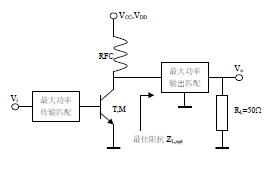
\includegraphics[scale=0.8]{A_PA}\newline
最大功率输出匹配 \newline
$V_{D, max} = 2V_{DD}$ \newline
$R_{L, opt} = \frac{V_{C, max} - V_{C, sat}}{I_{C, max}} \approx \frac{2V_{DD}}{I_{C,  max}}$\newline
\textbf{C类功放} \newline
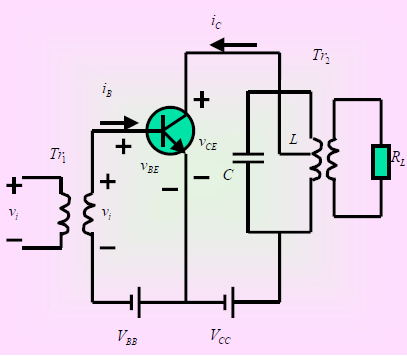
\includegraphics[scale=0.5]{C_PA}\newline
变压器耦合(阻抗匹配,单端转悬浮,直流隔离) \newline
电感部分接入(减少晶体管输出阻抗对谐振回路影响)\newline
$ v_o(t) = I_m \frac{\theta - sin\theta cos\theta}{\pi(1 - cos\theta)}R_L cos\omega t $\newline
$ I_m = g V_{im}(1 - cos\theta)$ \newline
$P_o = \frac{1}{2} I_{C1}V_{om} \quad P_s = I_{c0}V_{CC}$\newline
$\eta = \frac{1}{2}\frac{\alpha_1(\theta)}{\alpha_0(\theta)}\rho$ \newline
$\rho = \frac{V_{om}}{V_{CC}} $\newline
$ \theta \approx 60^{\circ}  -  70^{\circ} $\newline
$ V_{om} = I_{C1}R_L $ \newline
\textbf{吉尔伯特单元} \newline
BJT差分对:$ i_1 - i_2 = I_0 tanh\frac{v}{2v_T} $ \newline
单差分:$ i_d = i_1 - i_2 = (A + Bv_Y) tanh\frac{v_X}{2v_T} $\newline
$S_2(\omega t) = 2S_1(\omega t) - 1$\newline
$S_2(\omega t)  =  \frac{4}{\pi}cos\omega_Xt - \frac{4}{3\pi} cos 3\omega_Xt ...$ \newline
Gilbert:$ v_o = R_C I_0 tanh(\frac{v_X}{2v_T})tanh(\frac{v_Y}{2v_T}) $ \newline
\textbf{ 振荡器}
\newline
正反馈振荡器$H(s) = \frac{A(s)}{1 - A(s)F(s)}$ $A(j\omega_{osc})F(j\omega_{osc})=1$ \newline
必要条件:正反馈or负阻;至少两个极点。Q值越高,震荡频率越逼近LC谐振腔自由震荡频率。\newline
$V_i$小,$g_m = \frac{I_{c0}}{v_T}$;$V_i$大,$g_m = \frac{\overline{I}_0'}{V_{im}}$ \newline
稳幅措施:差分对,自动电平控制,负反馈,自给偏置\newline
稳定条件:$\frac{\partial|AF|}{\partial v_i}|_{平衡} < 0, \frac{\partial \phi_{AF}}{\partial v_i}|_{平衡} < 0$ \newline
起振条件:$|T| >1, \phi_T = 2n\pi$ 
平衡条件:$T(\omega_{osc}) = 1, \phi_T = 2n\pi$ \newline
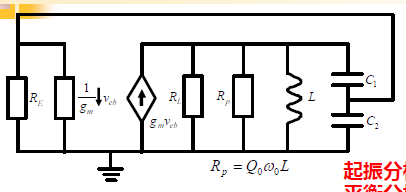
\includegraphics[scale=0.7]{CB}\newline
CB组态放大器小信号分析\newline
幅度条件 $ T = A_0 F \geq 1 $\newline
相位条件 $ \phi(\omega ) = 2n\pi $\newline
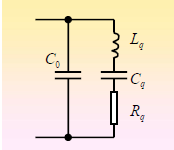
\includegraphics[scale=0.6]{crystal}\newline
晶振 $ f_q = \frac{1}{2\pi \sqrt{L_q C_q}} $\newline
$f_p = \frac{1}{2\pi \sqrt{\frac{C_q C_0}{C_q + C_0}}}$ \newline
串联型:高Q短路线 $f  = f_q$ \newline
并联型:电感 $f_q < f  < f_p$ \newline
n次泛音振荡: $ (n - 2)f_0 < f_ <  nf_0$ \newline

\textbf{标准调幅}\newline
 单音标准调幅:$v_{AM}(t) = V_{cm} cos\omega_c t + \frac{1}{2}m_aV_{cm}cos(\omega_c \pm \Omega)t$ \newline
 $P_t = P_c(1 + \frac{m_a^2}{2})$ \newline
 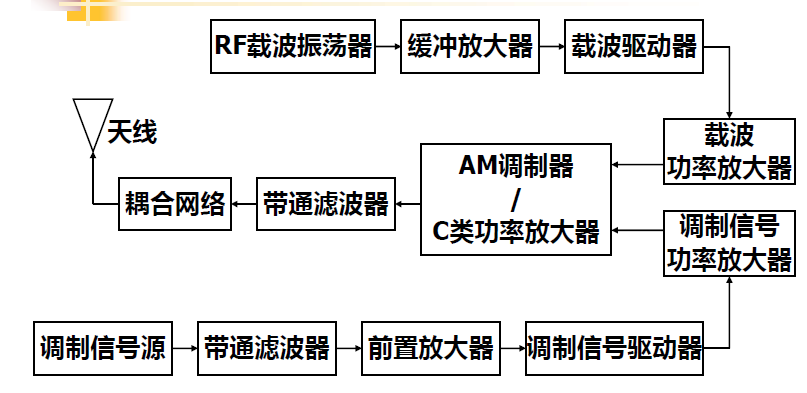
\includegraphics[scale=0.3]{高电平}\newline
 \textbf{相干解调}:AM信号与本地载波相乘 \newline
 非相干解调:平方律 \textbf{包络检波 }  \newline
 包络检波:$R_L C_L >> r_d C_L$ 对角切割失真 \newline
 \textbf{双边带调幅}\newline
 $v_{DSB}(t) = v_f(t) cos\omega_c t$ \newline
 \textbf{SSB}\newline
 $v_f'(t) = IFT(-jsgn(\omega)V_f(j\omega))$\newline
 上 $v(t) = \frac{1}{2}[v_f(t)cos\omega_ct - v_f'(t)sin\omega_ct]$ \newline
 下 $v(t) = \frac{1}{2}[v_f(t)cos\omega_ct + v_f'(t)sin\omega_ct]$ \newline
 多级滤波实现 $\delta = \frac{2F_{min}}{f_c}$\newline
 移相法实现  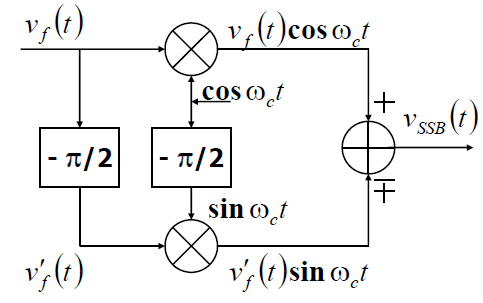
\includegraphics[scale=0.3]{移相}\newline
  频分复用:
    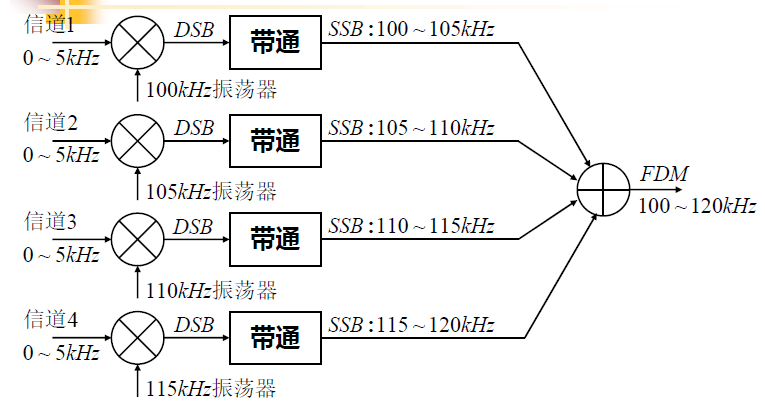
\includegraphics[scale=0.28]{FDM}\newline
 \textbf{ISB}\newline
 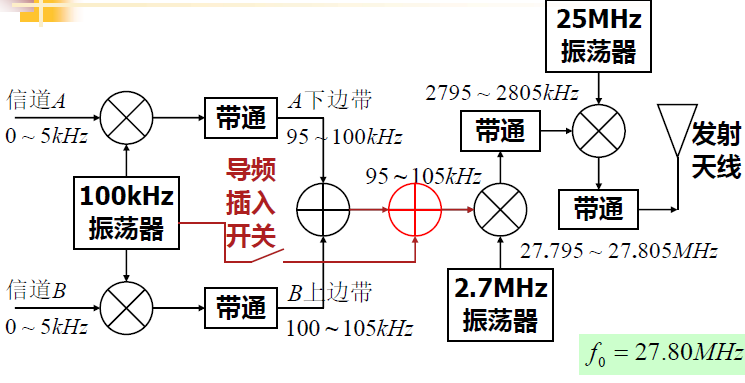
\includegraphics[scale=0.28]{ISB}\newline
 \textbf{正交AM}\newline
 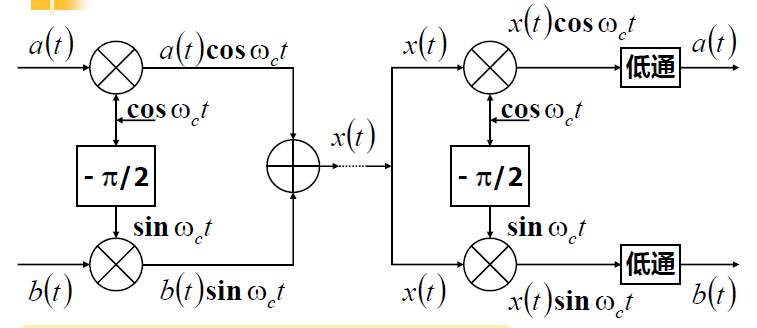
\includegraphics[scale=0.28]{OAM}\newline
 
 \textbf{收发结构}
Weaver收发结构:\newline
 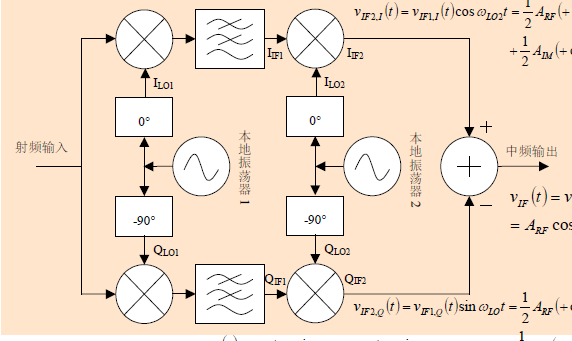
\includegraphics[scale=0.4]{Weaver}\newline
 外差收发结构: \newline
 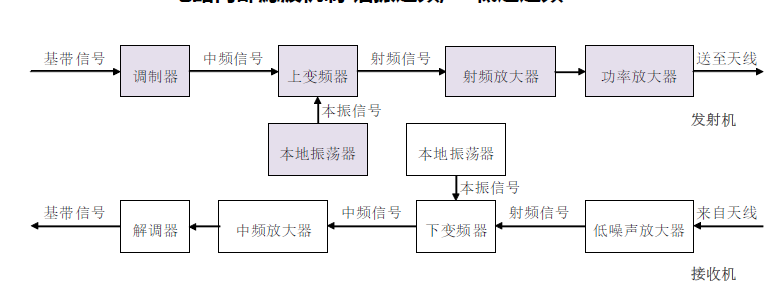
\includegraphics[scale=0.4]{外差接收}\newline
 外差结构:多个频段放大,固定中频高增益放大;多个频段分别滤波;\newline
 解决镜频干扰:二次变频;零中频;高中频;Hartley;Weaver结构; \newline
  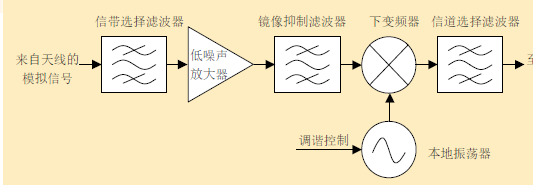
\includegraphics[scale=0.5]{镜像抑制结构}\newline
  上图为外差型镜像抑制接收机。 \newline
   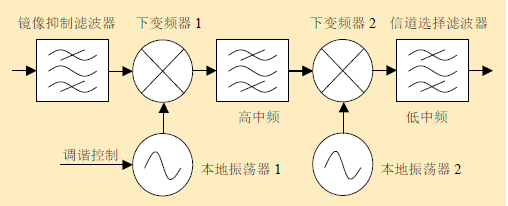
\includegraphics[scale=0.5]{二次变频}\newline
   上图为二次变频方案。\newline
   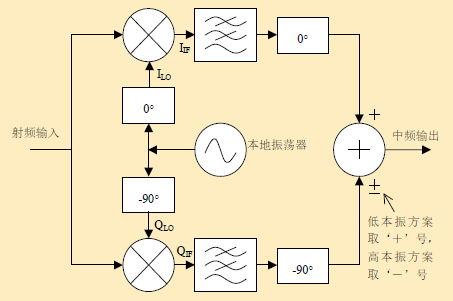
\includegraphics[scale=0.5]{Hartley}\newline
   上图为Hartley接收机。\newline
\textbf{调频与调相}
$v_{FM}(t) = V_{cm}cos(\omega_c t + K_F \int_0^t v_f(\tau)d\tau + \theta_0)$\newline
$v_{PM}(t) = V_{cm}cos(\omega_ct + K_pv_f(t) +\theta_0) $ \newline
$v_{FM}(t) = V_{cm}cos(\omega_c t + m_Fsin\Omega t + \theta_0)$ \newline
最大频偏: $ \Delta \omega = K_F V_{\Omega m}  $ \newline
$\omega_F(t) = \omega_c + K_Fv_f(t)$ \newline
 $m_F = \frac{\Delta \omega}{\Omega} = \frac{\delta f_m}{F}$ \newline
 FM复数:$exp(jm_Fsin\Omega t) = \sum_{n=-\infty}^{\infty} J_n(m_F)exp(jn\Omega t)$\newline
 $v_{FM}(t) = \sum_{n=-\infty}^{\infty}J_n(m_F)cos(\omega_c + n\Omega) t$ \newline
$J_{-n}(m_F) = (-1)^n J_n(m_F)$ \newline
$\sum_{n=-\infty}^{\infty}J_n^2(m_F) = 1$\newline
$J_n(m_F) \approx 0 \quad  if \  n > m_F + 1$ \newline
$BW_{FM} \approx 2(m_F + 1)F$ \newline 
窄带调频:$v_{FM}(t) = cos(\omega_c t ) - m_Fsin\Omega t sin\omega_ct$ \newline
宽带调频:$BW_{FM} \approx 2(m_F + 1)F = 2\Delta f_m + 2F$ \newline
\textbf{双音调制}\newline
$v_{FM}(t) = V_{cm}cos(\omega_c t + m_{F1}sin\Omega_1 t + m_{F2}sin\Omega_2 t + \theta_0)$\newline
$v_{FM}(t) = \sum_{n,k=-\infty}^{\infty} J_n(m_{F1})J_k(m_{F2})cos(\omega_c + n\Omega_1 + k\Omega_2)t$\newline
$\Delta f_m = \Delta f_{m, (max)}, F = F_{max}$ \newline
\textbf{噪声信号调制}\newline
$\Delta \theta_{peak} = \frac{V_{nm}}{V_{cm}}$ \newline
瞬时相位偏移 $\theta_n(t) = m_{Pn}sin(\Omega_n t + \theta_{n0})$\newline
瞬时频偏:$\Delta \omega_n(t) = \frac{V_{nm}}{V_{cm}}(\omega_n - \omega_c)cos((\omega_n - \omega_c)t + \theta_{n0})$\newline
最大频偏:$\Delta \omega_n = \frac{V_{nm}}{V_{cm}}(\omega_n - \omega_c) = m_{Pn}\Omega_n$ \newline
FM高端噪声分量产生解调噪声大于低端\newline
SNR: $SNR = \frac{\Delta \omega_s}{\Delta \omega_n}$\newline
预加重:调制前在发射机中加强FM信号频率高端振幅 \newline
去加重:解调后对调制信号频率高端进行衰减 \newline
\textbf{上变频调频方法}\newline
外差:
 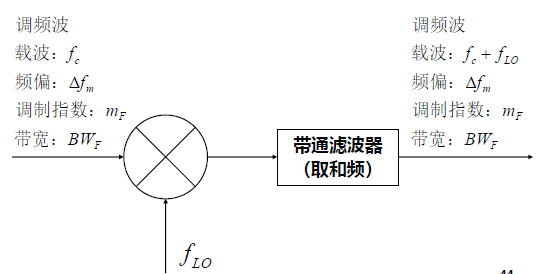
\includegraphics[scale=0.4]{外差}\newline
 倍频:
  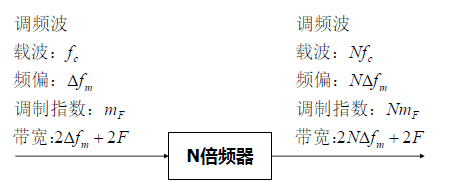
\includegraphics[scale=0.4]{倍频}\newline
  \textbf{变容二极管调频}\newline
  $f = \frac{1}{2\pi \sqrt{LC_j}}$ \newline
  $C_j = \frac{C_0}{(1 + \frac{v}{\phi})}^\gamma $ \newline
  二极管上电压:$V_B$,$v_f(t)$,$v_{osc}(t)$ \newline
  取$v = V_B + V_{\Omega m} cos\Omega t$ \newline
  则$C_j = \frac{C_0'}{(1 + m_c cos\Omega t)^\gamma}$ \newline
  $C_0' = \frac{C_0}{(1 + \frac{V_B}{\phi})^\gamma}$ \newline
  $m_C = \frac{V_{\Omega m}}{V_B + \phi} < 1$ \newline
  $f = f_c (1 + m_c cos\Omega t)^\frac{\gamma}{2}$ \newline
  频偏 $\Delta f_m = m_c f_c$ \newline
  灵敏度$S_F = \frac{\Delta f_m}{V_{\Omega m}} = \frac{f_c}{V_B + \phi}$ \newline
  非线性失真:$K_{f2} = \frac{1}{4}(\frac{\gamma}{2} - 1)m_c$ \newline
  载频漂移:$\frac{\Delta f_c}{f_c} = \frac{1}{8} \gamma (\frac{\gamma}{2} -1)m_c^2$ \newline
    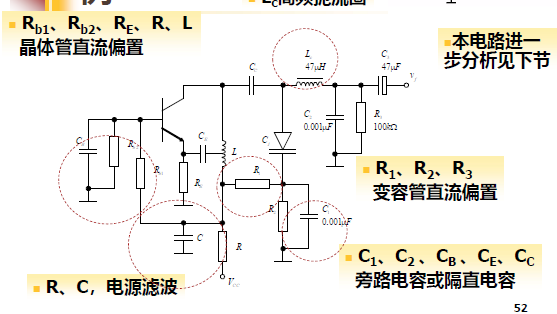
\includegraphics[scale=0.4]{FMdirect}\newline
 变容二极管稳频措施:部分接入,背靠背连接,晶振\newline
  增大直接调频绝对频偏方法:倍频,增大中心震荡频率\newline
 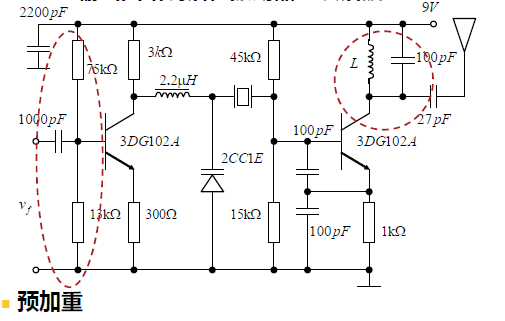
\includegraphics[scale=0.5]{晶振}\newline
\textbf{间接调频} \newline
 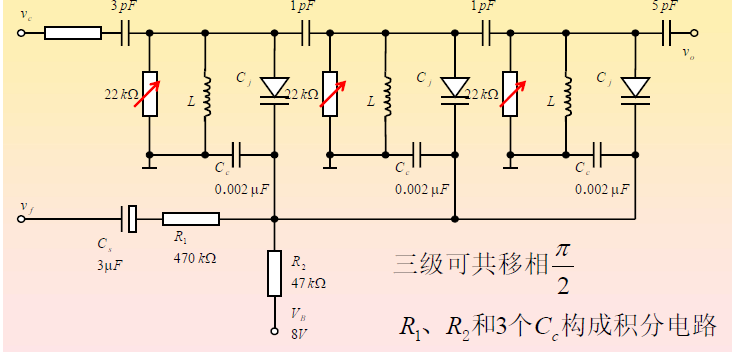
\includegraphics[scale=0.4]{间接调频}\newline
 直接调频中心频率稳定度低,频偏大。\newline
 大的频偏获得高的解调器解调性能\newline
 增大间接调频频偏方法:级联放大法 \newline
 
\textbf{调频波的解调\& 鉴频}\newline
二次变频外差接收机:
 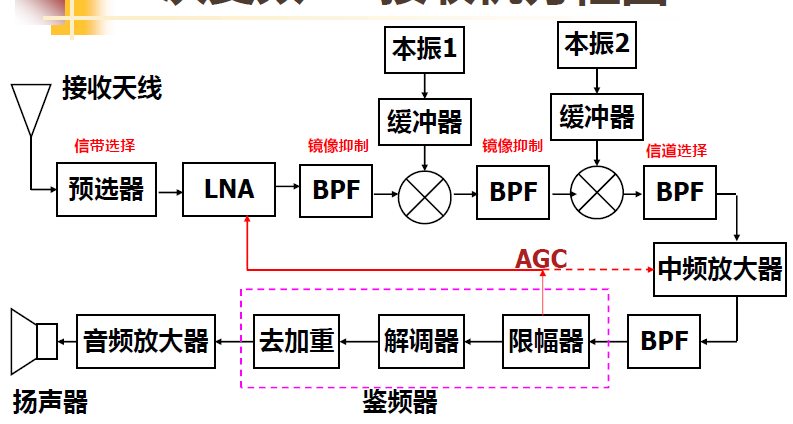
\includegraphics[scale=0.3]{外差1}\newline
\textbf{ 限幅鉴频}:消除寄生调幅,保证鉴频电压为等幅信号\newline
 鉴频器:$v_D$与输入信号频率$f$的关系\newline
 鉴频灵敏度:$S_D = \frac{\Delta V}{\Delta f}$ \newline
\textbf{ 斜率鉴频}:$\frac{dv_{FM}(t)}{dt} = (\omega_c + K_Fv_f(t))V_{cm}cos(w_c t + \phi(t))$ \newline
 斜率:$H(j\omega) = j\omega A_0$ \newline
 通过微分将调频波变换为调幅调频波,可以使用包络检波解决\newline
 单失谐回路:$A(\omega)= R_c(\omega - \omega_1)$ \newline
  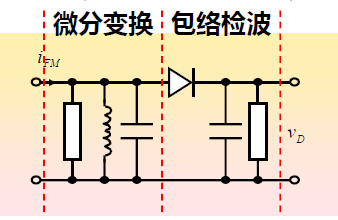
\includegraphics[scale=0.4]{单失谐}\newline
 双失谐回路:鉴频灵敏度增高 \newline
 \textbf{正交鉴频}\newline
 将调频波延时一段时间,令其相位变化与频率变化成正比。\newline
 $v_{FM}(t - \tau) = cos(\omega_c(t - \tau_0) + m_F sin \Omega (t - \tau_0))$ \newline
 $v_{FM}(t - \tau) \approx cos(\omega_c t + m_F sin \Omega t - m_F \Omega \tau_0 cos\Omega t - \omega_c \tau_0)$ \newline
  RLC并联谐振做延时电路:$\phi(\omega) = \frac{\pi}{2} - arctan Q(\frac{\omega}{\omega_0} - \frac{\omega_0}{\omega})$\newline
  $\phi(\omega) \approx \frac{\pi}{2} - 2Q\frac{\omega - \omega_0}{\omega_0} = \frac{\pi}{2} - \tau_0(\omega - \omega_0)$\newline
  采用乘法器+低通:$v_D(t) = \frac{1}{2}\tau_0 K_F v_f(t)$ \newline
  相加型鉴相器:延时后调频调相波与调频波相加,再用幅度检波 \newline 
  \textbf{PLL}\newline
    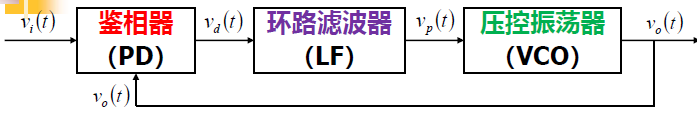
\includegraphics[scale=0.4]{PLL}\newline
  PD:将输入和输出信号的相位鉴别出来,转化为电压信号 \newline
  LF:对电压信号作低通滤波,滤除相位中高频噪声\newline
  VCO: 输出信号的相位跟踪输入信号的相位变化 \newline
  窄带跟踪:输出频率严格等于输入信号中心载频,用于\textbf{窄带调频} \newline
  调制跟踪:输出信号相位跟踪输入信号通带内相位变化,用于\textbf{宽带调频} \newline
  PD:$v_d(t) = K_d sin \phi_e(t) = K_d sin (\theta_1(t) - \theta_2(t)) $ \newline
  积分滤波器$H_F(s) = \frac{1}{1 + s\tau}$ 有源比例$H_F(s) = -\frac{1 + s\tau_2}{s\tau_1}$ \newline
  无源比例积分滤波$H_F(s) = \frac{1 + s\tau_2}{1 + s(\tau_1 + \tau_2)}$ 直通 $H(s) = 1$ \newline
  VCO:$\omega_o(t) = \omega_{o0} + K_\omega v_p(t)$ \newline
  固有积分$\frac{1}{s}$: $\phi_o(t) = \omega_{o0}t + K_\omega \int_{0}^{t}v_p(\tau)d\tau$ \newline
   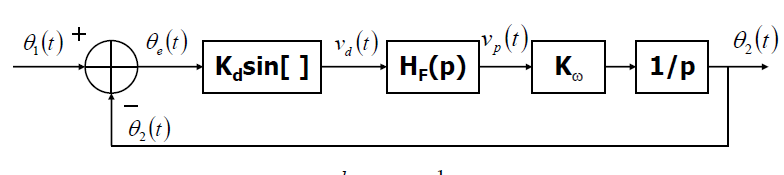
\includegraphics[scale=0.4]{PLL数学}\newline
  $\theta_e(t) = \theta_1(t) - \theta_2(t)$ $K_p = K_dK_w$ \newline
  环路方程$\frac{d\theta_e(t)}{dt} = \frac{d\theta_1(t)}{dt} - K_p(H_F(p)sin \theta_e(t))$ \newline
  直流分析:$\phi_{e \infty} = arcsin(\frac{\omega_{i0} - \omega_{o0}}{K_pH_F(0)})$ \newline
  $v_i(t) = V_{im}sin(\omega_{i0}t + \theta_{i0})$\newline
  $v_{o\infty}(t) = V_{om} cos(\omega_{i0}t + \theta_{i0} - \phi_{e\infty})$ \newline
  相位差中默认存在一个$\frac{\pi}{2}$直流分量(相乘鉴相的要求) \newline
  捕获带:$\Delta \omega_{max} = min(A_{F0}K_p, \Delta \omega_{VCO})$ \newline
  交流分析:$\phi_o(t) = \omega_{i0}t + \theta_{i0} - \phi_{e \infty} + \theta_{om}sin(\Omega t + \psi)$ \newline
  $\omega_o(t) = \omega_{i0} + \theta_{om}\Omega cos(\Omega t + \psi)$ \newline
  $| H_F(j\Omega)| = \frac{\theta_{om}}{\theta_{im}}, \psi = arg(H(j\Omega))$ \newline
  正弦鉴相小信号:$v_d(t) = K_d sin\phi_{e \infty} + K_d cos \phi_{e \infty}  \Delta \phi_e(t)$ \newline
  $\phi_e(t) = \phi_{e \infty} - K_\omega K_d cos \phi_{e \infty} \frac{1}{p} \cdot  H_F(p) \cdot  \Delta \phi_e(t)$ \newline
  $H_e(s) = \frac{s}{s + K_\omega K_d' H_F(s)}, K_d' = K_d cos\phi_{e \infty}$ \newline
  $H(s) = \frac{K_\omega K_d' H_F(s)}{s + K_\omega K_d' H_F(s)}$ \newline
  一阶PLL:$H(s) = \frac{K_\omega K_d'}{s + K_\omega K_d'} = \frac{\omega_0}{s + \omega_0}$ \newline
  二阶RC PLL: $H_F(s) = \frac{1}{1 + s\tau}$ $K_{ps} =  K_\omega K_d cos\phi_{e \infty}$ \newline
  $H(s) = \frac{K_{ps} / \tau}{s^2 + s / \tau + K_{ps}/\tau} = \frac{\omega_n^2}{s^2 + 2\xi\omega_ns + \omega_n^2}$ \newline
  $\omega_n = \sqrt{\frac{K_ps}{\tau}}$ $\xi = \frac{1}{2\sqrt{K_{ps}\tau}}$ \newline
  无源比例$\omega_n = \sqrt{\frac{K_ps}{\tau_1 + \tau_2}}$ $2\xi\omega_n = \frac{1 + K_{ps}\tau_2}{\tau_1 + \tau_2}$ \newline
  有源比例$\omega_n = \sqrt{\frac{K_ps}{\tau_1}}$ $2\xi\omega_n = K_{ps}\frac{\tau_2}{\tau_1}$ \newline
  调制跟踪:$\Omega$位于LF通带以内,则输出为一调角波,为调制跟踪。\newline
  载波跟踪:$\Omega$位于通带之外,输出载波信号,为载波跟踪。 \newline
  
  \textbf{PLL稳定性} 极点全部位于左半平面 $H(s) = \frac{H_o(s)}{1 + H_o(s)}$\newline
  Baud准则: $\phi(\omega_k) = \pi, |H_o(j\omega_k)| < 0dB$ $H_o(j\omega_p) = 0dB,  |\phi(\omega_p)| < \pi$ \newline
  一阶锁相环稳定,$PM = 90^{\circ}$ \newline
  二阶锁相环:$H(s) = \frac{K_p}{s(1 + s\tau)}$ $PM = 90^{\circ} - atan \sqrt{\frac{\sqrt{1 + 4 K_p^2\tau^2} - 1}{2}} $    $K_p \tau = 0.515 \quad PM = 65^{\circ}$\newline
  \textbf{PLL非线性}同步带:$\Delta \omega_H = K_p H_F(0) = K_d K_\omega H_F(0)$ \newline
  捕捉带$\Delta \omega_P$ 块捕带$\Delta \omega_c$ $\Delta \omega_c < \Delta \omega_P < \Delta \omega_H$ \newline
  一阶PLL:$\frac{d \phi_e(t)}{dt} + K_p sin \phi_e(t) = \omega_{i0} - \omega_{o0} = \Delta \omega_i$ \newline
  此时$K_p = K_d K_\omega$ $\phi_e = arcsin\frac{\Delta \omega_i}{K_p}$\newline
   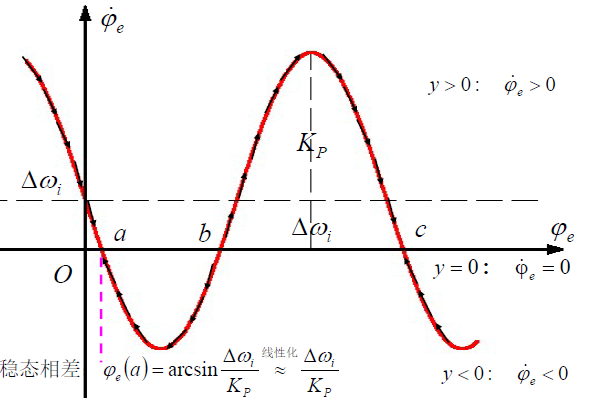
\includegraphics[scale=0.4]{相图}\newline
 起始频差超出捕捉带则VCO平均振荡频率向$f_i$逼近:\textbf{频率牵引} \newline
 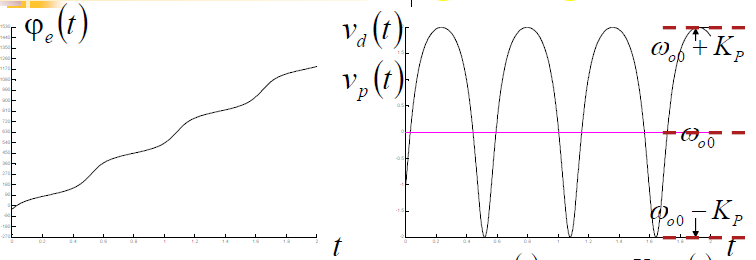
\includegraphics[scale=0.4]{频率牵引}\newline
 直流分量$V_p = K_d[\frac{\Delta \omega_i}{K_p} - \sqrt{(\frac{\Delta \omega_i}{K+p})^2 - 1}]$ \newline
 \textbf{捕捉}二阶环捕捉分为‘频率牵引’和‘相位锁定’。$\Delta \omega_c = s\xi\omega_n$\newline
 加速捕捉策略: 扩大带宽, 减小频差, 引入AFC \newline
 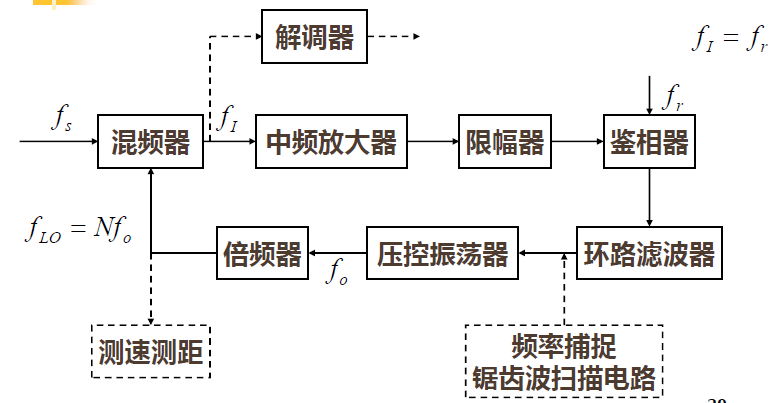
\includegraphics[scale=0.4]{锁相接收1}\newline
上图为 窄带跟踪环接收策略 \newline
 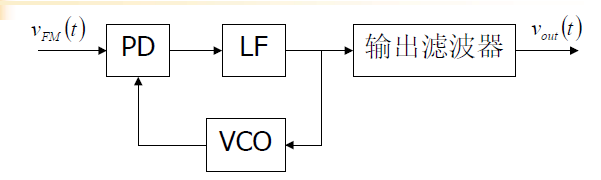
\includegraphics[scale=0.4]{锁相鉴频}\newline
上图为 锁相鉴频策略 \newline
\textbf{AFC}\newline
 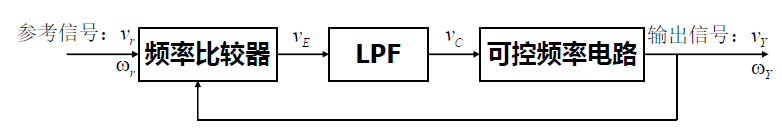
\includegraphics[scale=0.4]{AFC}\newline
 $T(s) = \frac{K_dK_oH_F(s)}{1 +K_dK_oH_F(s)}$ $T_e(s) = \frac{1}{1 +K_dK_oH_F(s)}$ \newline
 $v_e(t) = K_d(\omega_i - \omega_o) = K_d \omega_e$ $\omega_Y = K_o v_C + \omega_{Y0}$ \newline
频率阶跃 $\delta_\omega = \frac{\Delta \omega}{1 + K_dK_oH_F(0)}$\newline

\end{multicols*}
\end{document}
